
% Article - значит без глав, только секции
\documentclass{article}
\usepackage{lmodern}
% Задаем шрифты
\usepackage{fontspec}
\setmainfont[Scale=1.4]{Times New Roman} % Главный шрифт
\setmonofont[Scale=1.0]{Consolas} % Моноширинный шрифт

% Поддержка русского языка (переносов, орфографии)
\usepackage{polyglossia}
\setmainlanguage{russian} % Ставим русский главным
\setotherlanguage{english} % Английский второстепенным

% Отступы по ГОСТу
\usepackage{geometry}
\geometry{
	a4paper,
	left=3cm,
	top=2cm,
	bottom=2cm,
	right=1cm,
}

% Можно вставлять скрипты на Lua (компилить через lualatex)
%\usepackage{luacode}

% Example
% \begin{luacode}
% tex.print(math.random())
% \end{luacode}

\usepackage{listings}
\lstset{
  basicstyle=\ttfamily,
  keywordstyle=\ttfamily,
  stringstyle=\ttfamily,
  commentstyle=\ttfamily,
  breaklines=true,
  keepspaces=true,
  extendedchars=\true
}


\usepackage{python}


%%% ТИТУЛЬНИК %%%
%%%%%%%%%%%%%%%%%

\begin{document}
% Отключаем нумерацию страниц
\pagenumbering{gobble}
\begin{center}

МИНИСТЕРСТВО ОБРАЗОВАНИЯ И НАУКИ РОССИЙСКОЙ ФЕДЕРАЦИИ
НОВОСИБИРСКИЙ ГОСУДАРСТВЕННЫЙ ТЕХНИЧЕСКИЙ УНИВЕРСИТЕТ
ФАКУЛЬТЕТ АВТОМАТИКИ И ВЫЧИСЛИТЕЛЬНОЙ ТЕХНИКИ
КАФЕДРА ВЫЧИСЛИТЕЛЬНОЙ ТЕХНИКИ

\vspace{\fill}
{\bfseries \Large Расчетно-графическая работа}

{\itshape по дисциплине <<Современные информационные технологии>>}

на тему <<Одностраничное Web-приложение>>

\vspace{\fill}

\begin{flushleft}
\begin{tabular}{ l l }
Студент & Кузьмин Д.С. \\
Группа & АВТ-318 \\
Преподаватель & Васюткина И.А. \\
\end{tabular}
\end{flushleft}

\vspace{\fill}
Новосибирск 2015 г.
\end{center}
\pagebreak

% Включаем нумерацию страниц
\pagenumbering{arabic}

%%% СЕКЦИИ %%%
%%%%%%%%%%%%%%

\section*{Цель работы}

Разработать одностраничное веб-приложение с использованием веб-фрейворка Vaadin для отображения 
информации о погоде в различных городах, курсе валют и кол-ве посещений страницы приложения


\section*{Задание}

\begin{enumerate}

\item При создании приложения использоть веб-фрейворк Vaadin для создания интерфейса и взаимодействия между клиентом и сервером.
\item Реализовать получение и парсинг данных прогноза погоды на текущий и завтрашний день с сервиса ForecastIO
\item Реализовать получение и парсинг данных о курсах валют (доллар США, евро) с сайта ЦентроБанка России
\item Реализовать учет числа посещений страницы во время работы приложения (уникальные посетители, общее число посещений)
\item Добавить возможность обновлять данные из пунктов выше вручную по нажатию кнопки без перезагрузки страницы
\item Показывать IP-адрес пользователя, находящегося на странице
\item Показывать на странице время последнего обновления данных
\item Хранить информацию о посещениях из NoSQL БД Mongo

\end{enumerate}

\section*{Описание работы}

Была реализована следующая структура классов:

\begin{figure}[h]
\centering
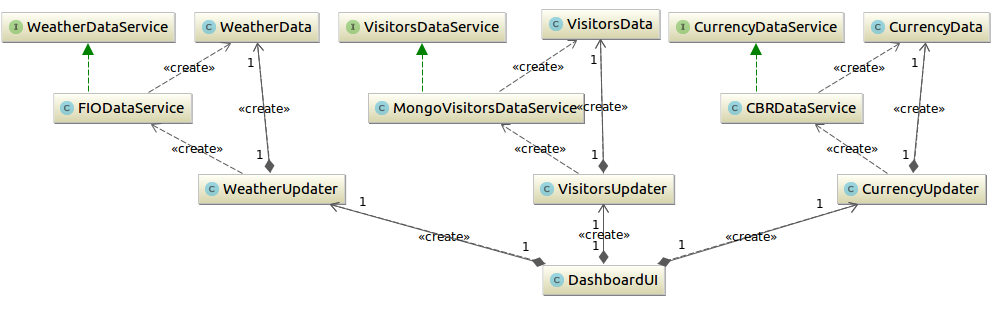
\includegraphics[width=\textwidth]{uml}
\caption{Диаграмма классов проекта}
\end{figure}

Краткое описание реализованных абстракций:
\begin{itemize}
\item Классы типа <<DataService>> работают непосредственно с источниками данных (база данных, сторонние сервисы). Результатом их работы является класс с полезной информацией типа <<Data>>
\item Классы типа <<Data>> содержат в себе информацию, необходимую и достаточную для ее отображения в графическом интерфейсе без дополнительных запросов к посторонним модулям.
\item Классы типа <<Updater>> реализуют функционал обновления графических компонентов, предобрабатывая и передавая информацию из классов типа <<Data>> этим компонентам.
\item Класс DashboardUI является корневым классом проекта. Он напрямую взаимодействует с фреймворком Vaadin - инициализирует интерфейс и является насленидком его класса шаблона. Этот класс имеет внутренний класс DashboardUIServlet, который является 
наследником HttpServlet и привязывается к контейнеру сервлетов аннотацией фреймворка.
\end{itemize}

Привозникновении непредвиженных ситуаций, пользователю сообщается 
об ошибке в сплывающей панели.

Представление информации на стороне клиента:

\begin{figure}[h]
\centering
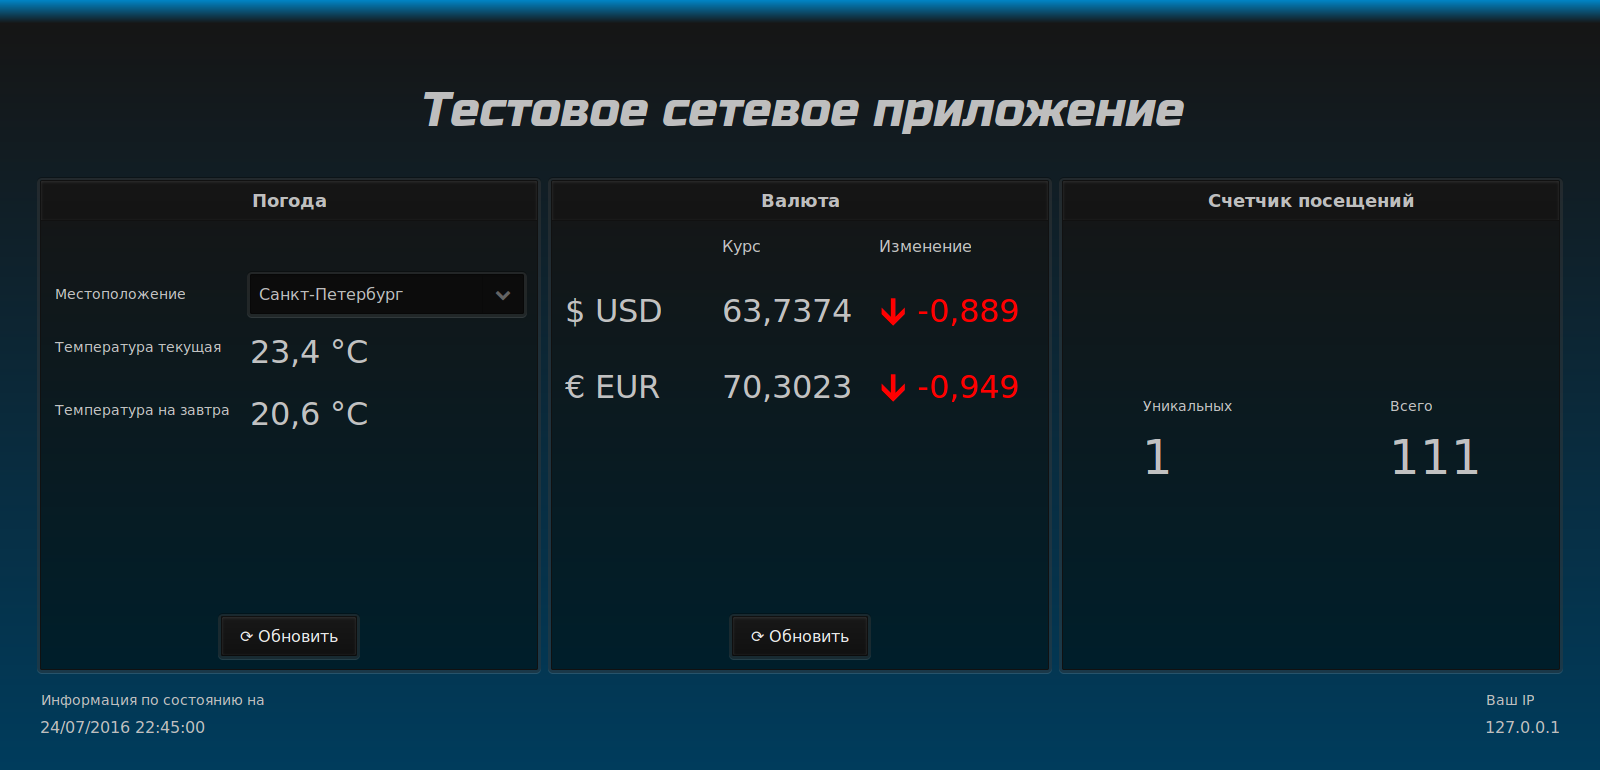
\includegraphics[width=\textwidth]{screenshot}
\caption{Скриншот приложения}
\end{figure}

\section*{Вывод}
Было реализовано одностраничное приложение для отображения информации по погоде, курсе валют и количестве посещений.
Как основа использовался веб-фреймворк Vaadin. Данная технология 
полностью реализует процесс разработки клиентской стороны приложения
и процесс обмена информацией между браузером клиента и сервером Tomcat8, что существенно ускоряет процесс разработки.
\pagebreak

\section*{Список литературы}
\begin{enumerate}
	\item Book of Vaadin: [Электронный ресурс]. URL: https://vaadin.com/book. (Дата обращения: 28.12.2016).
\end{enumerate}	

\pagebreak
\section*{Приложение А. Листинг программы}

\lstinputlisting[title=\large{ExceptionForUser.java}]{src/main/java/com/xotonic/dashboard/ExceptionForUser.java}
\lstinputlisting[title=\large{CBRDataService.java}]{src/main/java/com/xotonic/dashboard/currency/CBRDataService.java}
\lstinputlisting[title=\large{CurrencyData.java}]{src/main/java/com/xotonic/dashboard/currency/CurrencyData.java}
\lstinputlisting[title=\large{CurrencyDataService.java}]{src/main/java/com/xotonic/dashboard/currency/CurrencyDataService.java}
\lstinputlisting[title=\large{CurrencyUpdater.java}]{src/main/java/com/xotonic/dashboard/ui/CurrencyUpdater.java}
\lstinputlisting[title=\large{DashboardUI.java}]{src/main/java/com/xotonic/dashboard/ui/DashboardUI.java}
\lstinputlisting[title=\large{VisitorsUpdater.java}]{src/main/java/com/xotonic/dashboard/ui/VisitorsUpdater.java}
\lstinputlisting[title=\large{WeatherUpdater.java}]{src/main/java/com/xotonic/dashboard/ui/WeatherUpdater.java}
\lstinputlisting[title=\large{MongoVisitorsDataService.java}]{src/main/java/com/xotonic/dashboard/visitors/MongoVisitorsDataService.java}
\lstinputlisting[title=\large{VisitorsData.java}]{src/main/java/com/xotonic/dashboard/visitors/VisitorsData.java}
\lstinputlisting[title=\large{VisitorsDataService.java}]{src/main/java/com/xotonic/dashboard/visitors/VisitorsDataService.java}
\lstinputlisting[title=\large{Cities.java}]{src/main/java/com/xotonic/dashboard/weather/Cities.java}
\lstinputlisting[title=\large{FIODataService.java}]{src/main/java/com/xotonic/dashboard/weather/FIODataService.java}
\lstinputlisting[title=\large{OpenWeatherMap.java}]{src/main/java/com/xotonic/dashboard/weather/OpenWeatherMap.java}
\lstinputlisting[title=\large{WeatherData.java}]{src/main/java/com/xotonic/dashboard/weather/WeatherData.java}
\lstinputlisting[title=\large{WeatherDataService.java}]{src/main/java/com/xotonic/dashboard/weather/WeatherDataService.java}


\end{document}
